\documentclass{standalone}

\usepackage[euler-digits]{eulervm}

\usepackage{tikz}
\tikzset{every node/.style={circle,draw,minimum size=6mm,inner sep=0pt}}
\tikzset{t/.style={rectangle}}

\begin{document}
    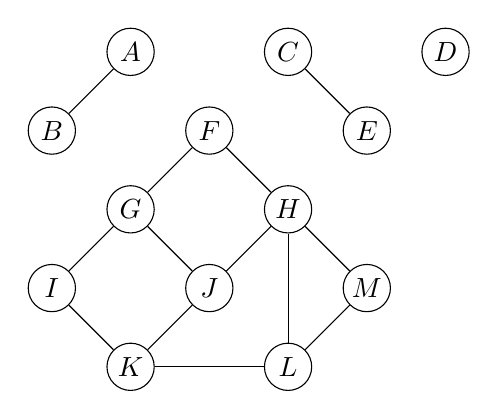
\begin{tikzpicture}[font=\sffamily]
      \node (A) at (-1,3) {$A$}; 
      \node (B) at (-2,2) {$B$}; 
      \node (C) at (1,3) {$C$}; 
      \node (D) at (3,3) {$D$}; 
      \node (E) at (2,2) {$E$}; 
      \node (F) at (0,2) {$F$}; 
      \node (G) at (-1,1) {$G$}; 
      \node (H) at (1,1) {$H$}; 
      \node (I) at (-2,0) {$I$}; 
      \node (J) at (0,0) {$J$}; 
      \node (K) at (-1,-1) {$K$}; 
      \node (L) at (1,-1) {$L$}; 
      \node (M) at (2,0) {$M$}; 
      \foreach \a/\b in {A/B,C/E,F/G,F/H,G/I,G/J,H/J,H/L,H/M,I/K,J/K,K/L,L/M}
        \draw (\a) -- (\b);
    \end{tikzpicture}
\end{document}
